\documentclass[twoside,twocolumn]{article}

\usepackage[version = 4]{mhchem} %chem symbols and equations
\usepackage{graphicx} %graphics
\usepackage{amssymb} %math symbols
\usepackage{amsmath} %math equations
\usepackage{hyperref} %create hyperlinks: \href{link}{Word to click on}

\usepackage[sc]{mathpazo} % Use the Palatino font
\usepackage[T1]{fontenc} % Use 8-bit encoding that has 256 glyphs
\linespread{1.05} % Line spacing - Palatino needs more space between lines
\usepackage{microtype} % Slightly tweak font spacing for aesthetics
\usepackage[english,spanish]{babel} % Language hyphenation and typographical rules

\usepackage[hmarginratio=1:1,top=27mm,columnsep=20pt,left=15mm,right=15mm]{geometry} % Document margins
\usepackage[hang,small, labelfont=bf,up]{caption} % Custom captions under/above floats in tables or figures
\usepackage{enumitem} % Customized lists
\setlist[itemize]{noitemsep} % Make itemize lists more compact

\usepackage{abstract} % Allows abstract customization
\renewcommand{\abstractnamefont}{\normalfont\bfseries} % Set the "Abstract" text to bold

\usepackage{titlesec} % Allows customization of titles
\titleformat{\section}[block]{\large\centering\bfseries}{\thesection.}{1em}{} % Change the look of the section titles
\titleformat{\subsection}[block]{\bfseries}{\thesubsection.}{1em}{} % Change the look of the section titles

\usepackage{fancyhdr} % Headers and footers
\pagestyle{fancy} % All pages have headers and footers
\fancyhead{} % Blank out the default header
\fancyfoot{} % Blank out the default footer
\fancyhead[C]{Physical Chemistry $\bullet$ Oct 2019 $\bullet$ Vol. XXI, No. 1} % Custom header text
\fancyfoot[RO,LE]{\thepage} % Custom footer text

\usepackage{titling} % Customizing the title section

\renewcommand{\maketitlehookd}{%
\begin{abstract}
\noindent
En este documento voy a escribir algunos detalles de los avances en el trabajo con el Profesor Guillermo Restrepo, as\'i como preguntas e ideas que puedan surgir en el camino. 
\end{abstract}
}



\begin{document}

\title{Avances del trabajo con Prof. Guillermo Restrepo} 

\author{%
\textsc{Andr\'es C. Marulanda}\thanks{Corresponding author} \\[1ex]
\normalsize Universidad de Antioquia \\ % Your institution
\normalsize \href{mailto:correoAndres}{acamilo.marulanda@udea.edu.co} % Your email address
}


\maketitle


\section{Introducci\'on}
\label{sec:intro}

El objetivo es obtener un algoritmo capaz de hacer predicciones utilizando datos de sustancias actuales (hasta cierta fecha). Para esto, el objetivo es leer el sistema peri\'odico (PS) de la misma manera que lo vi\'o Mendeleev para hacer sus predicciones; esto es, saber en qu\'e partes la similaridad es vertical, en cuales es horizontal, diagonal, etc, y c\'omo hacer predicciones sobre nuevos compuestos con este conocimiento.
Inicialmente pensamos en redes neuronales convolucionales que tomen como input datos representados en un esquema de tabla peri\'odica, similar a lo que hicieron en \cite{CNN_dH}.

Adicionalmente podemos intentar interpretar (disecar) la red neuronal. Esto lo podemos hacer de la misma manera que se hace para las redes que se ocupan de tareas de visi\'on artificial, por lo que podemos ver cada uno de los filtros y como estos se comportan a medida que los inputs var\'ian. 

Esto podr\'ia dar la informaci\'on de c\'omo leer alg\'un PS, sea el de Mendeleev o cualquier otro, pues nos podr\'ia dar informaci\'on de en qu\'e partes del PS importan las similaridades verticales, diagonales, etc. 
El c\'odigo desarrollado hasta este momento toma como entrada un custom PS, esto es, un PS escrito por el usuario. Este puede ser el de Mendeleev, el desarrollado por el grupo de Prof. Restrepo o cualquier otro. La utilidad de esto recae en que puede darnos alguna idea de c\'omo es la convergencia del algoritmo con diferentes PSs, y con esto evaluar el contenido de informaci\'on de cada uno. As\'i podr\'ian compararse algoritmos para leer el PS de Mendeleev contra PS organizados aleatoriamente, entre otros.

Hasta este punto se tendr\'ia un "Mendeleev robot", al cual podemos examinar para ver como toma decisiones.

Si logramos esto, digamos, para el PS (y sustancias) de 1868, podemos pensar en hacer lo mismo para varios a\~nos alrededor de \'este y evaluar como era la capacidad predictiva del PS de este a\~no. Esto podr\'ia dar alguna evidencia de que 1868 fue el a\~no (o la \'epoca) m\'as apropiada para la creaci\'on del PS. En este punto cabe aclarar que ya se tiene listo un art\'iculo sobre este tema, donde se muestra que el PS estaba listo para ser formulado desde 1840.

M\'as adelante podr\'ian entrenarse sistemas similares para no s\'olo predecir probabilidad de existencia, sino tambi\'en para aproximar algunas propiedades de compuestos por reemplazamiento de un elemento. Esto podr\'ia ser de utilidad, por ejemplo, si se buscara predecir propiedades de los compuestos formados con elementos desconocidos hasta la fecha, que es precisamente lo que hizo Mendeleev con el esta\~no y otros. 

Se quiere utilizar sustancias mas PS como entrada para un algoritmo. Digamos, por ejemplo, que para las sustancias $\ce{R-Na_n}$ y $\ce{R-K_n}$ existen propiedades medidas. Luego, el objetivo del algoritmo ser\'a predecir esta propiedad para, p.e., $\ce{R-Fe_n}$ (Fe o cualquier otro). Esta propiedad puede ser alguna propiedad experimental, o probabilidad de existencia, etc.

El algoritmo se encarga en el primer caso de aproximar la funci\'on

\begin{equation}
\label{eq:eq1}
 f(R-x_n) = f( x, existent R-Y_n , PS )
\end{equation}

Y en el segundo caso de calcular la siguiente probabilidad:

\begin{equation}
\label{eq:eq2}
P ( existe R-X |  existe R-Y  + PS )
\end{equation}

Con X cualquier elemento conocido en la \'epoca, Y un elemento tal que $\ce{R-Y_n}$ existe en la \'epoca considerada y PS es el sistema peri\'odico de esa \'epoca.

Del algoritmo se espera que eval\'ue la similaridad entre X y Y, de manera que si estos son similares, la probabilidad de que exista un compuesto resultado de la sustituci\'on de estos elementos deber\'ia de ser alta, y sus propiedades similares. Esta informaci\'on de similaridad deber\'ia de poder encontrarse, por supuesto, en el PS. 


\section{Tratamiento de datos}
\label{sec:sec2}

El input puede ser un esquema de la tabla peri\'odica (PT), construido de la siguiente manera.

Suponga que existe un conjunto de elementos A = \{$A_i$\} y un fragmento de sustancia R tal que $\ce{R-A_n}$ existe en la \'epoca considerada. Entonces en nuestra representaci\'on, en la posici\'on de cada uno de los elementos de A en la PT se asignar\'a un valor de 1. De otra manera, el valor ser\'a de 0. Ahora bien, la pregunta es: existe la sustancia R-Y, para un elemento conocido Y? 
Este elemento Y tendr\'a un valor de -1 en la representaci\'on de la PT (PTR).
En caso que R-Y exista en esta \'epoca, el label (y) es igual a 1, de otra manera es igual a 0. Un ejemplo de esta PTR se da en la figura \ref{fig:fig1}, en la que se indica que los elementos K, Mg, O, S comparten una composici\'on R-X$_n$ en com\'un, esto es, el compuesto RX$_n$ existe en el conjunto de datos con X = K, Mg, O, S. Adicionalmente se indica la pregunta: Existe el compuesto R-Br$_n$?

\begin{figure}[h!]
	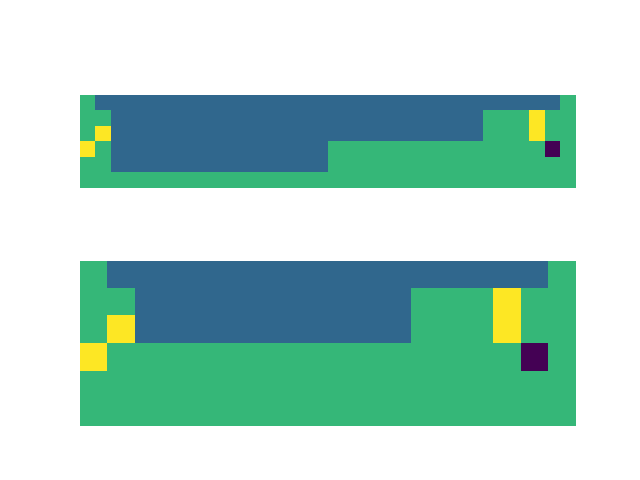
\includegraphics[width=\linewidth]{ex1TPR.png}
	\caption{Representaci\'on de la tabla peri\'odica (PTR). (Arriba/abajo) representaci\'on incluyendo/sin serie de lant\'anidos.}
	\label{fig:fig1}
\end{figure}

Similarmente, en el caso de la predicci\'on de propiedades, estos valores se intercambian por los valores reales de las sustancias consideradas.

\subsection{Generaci\'on de los datos}

Se encuentra cada fragmento $\ce{R_n}$ en el dataset, luego se encuentra una lista de elementos A = {$A_i$} tal que $\ce{R-A_n}$ exista para cada n; lo que produce una cantidad N($\ce{R_n}$) de fragmentos $\ce{R_n}$ y por lo tanto de PTRs. El nuevo dataset contiene la informaci\'on correspondiente a las similaridades entre elementos, as\'i como los $\ce{R_n}$ con los que se combinan.

En este punto se hace un an\'alisis exploratorio de los datos (EDA), para lo cual se pueden tener consideraciones que se exponen en la siguiente secci\'on.

El tama\~no del dataset para alimentar al algoritmo efectivamente es expandido al incluir la informaci\'on sobre las sustancias que quieren predecirse, esto es, mediante un "labeling" del dataset. 
Para cada PTR puede sugerirse al algoritmo que ejecute la predicci\'on de propiedades para X elementos, lo que incrementa el tama\~no del dataset a N($\ce{R_n}$)*X.

\subsection{Algoritmo}
Suponga que tiene un compuesto R-X$_n$, con $n \geq 1$. Consideramos como un nuevo R$'$ la combinaci\'on RX, de manera que tenemos un ``nuevo compuesto'' RX-X$_{n-1}$ = R$'$-X$_{n-1}$. Puede continuarse de esta manera hasta agotar n, esto es, pueden crearse n-1 nuevos R$'$ para un total de $n$ Rs diferentes a partir de uno s\'olo de los elementos de uno de los compuestos. Con esto se genera una cantidad de $\ce{R_n}$s igual a la suma de todos los sub\'indices de cada elemento en todos los compuestos.

Naturalmente esto aumenta la cantidad de datos disponibles, pues se explota cada uno de los sub\'indices de cada elemento en cada f\'ormula molecular, lo cual es una ventaja en t\'erminos computacionales pues puede llevar a la reducci\'on del overfitting y otros problemas que se encuentran durante la producci\'on de modelos en machine learning (ML).

Por ejemplo, las f\'ormulas $\ce{C6BrCl2H3}$ y $\ce{C6Cl3H3}$ pueden compararse as\'i: pueden escribirse como $\ce{C6Cl2H3-Br}$ y $\ce{C6Cl2H3-Cl}$. Esto lleva a que $\ce{Cl}$ y $\ce{Br}$ comparten este ligando en com\'un, mostrando una similaridad que no se expresa con m\'etodos m\'as simples.


\section{An\'alisis de datos}

Una vez se tengan las PTR, se procede con el an\'alisis de los datos. Esta secci\'on se divide en dos: an\'alisis exploratorio (EDA), en el que se quiere obtener datos estad\'isticos y medidas generales del dataset, y modelaci\'on, donde se quiere intentar dar estructura, significado y utilidad a los datos generados. 

\subsection{EDA}

Ah pues aqu\'i se hacen cosas :|

\subsection{Modelaci\'on}
\subsubsection{Clustering}
En esta secci\'on se pretende utilizar m\'etodos de ML y los datos obtenidos para dar estructura, significado y utilidad a los datos generados.
El primer m\'etodo que puede usarse es clustering. En este se utilizan algoritmos para encontrar clusters de elementos (no estrictamente en el sentido qu\'imico) similares dada una representaci\'on. En este caso al aplicarlo a las PTR, buscamos las combinaciones de elementos que m\'as ocurren en estas. Debe recordarse que cada PTR representa a una sustancia por medio de los elementos que la componen y son reemplazables entre s\'i, lo que sugiere similaridad. Si los elementos de uno conjunto son en verdad similares, esto se repetir\'a constantemente a trav\'es de todas las sustancias consideradas, por lo que los clusters con mayor n\'umero de PTRs corresponder\'an a los grupos de similaridad m\'as evidentes. En general lo que se obtiene son clusters representado grupos de similaridad entre elementos, lo que en la visi\'on del PS como hipergrafos ordenados se nombra ''hyperedges''.

\subsubsection{Algoritmo predictor}
La idea inicialmente es utilizar redes neuronales para aproximar la funci\'on descrita por las ecuaciones \ref{eq:eq1} y \ref{eq:eq2}. La arquitectura a usar es uno de los grandes problemas debido a que no existe una \'unica manera de obtener una \'optima y usualmente la aproximaci\'on es una heur\'istica, donde se sugiere c\'omo se quiere que el algoritmo lea los datos. Adicionalmente en las arquitecturas convencionales existen limitaciones en t\'erminos del tipo de datos que pueden usarse, por lo que esto debe pensarse detenidamente. Por ejemplo, las redes convolucionales (CNN) se usan para la lectura de im\'agenes; si se quisiera dar como input una imagen mas un vector, tendr\'ia que pensarse en algo m\'as.

Un problema de nuestra representaci\'on, sin embargo, es que no conserva nada de la informaci\'on del fragmento R ni del sub\'indice n, sino s\'olo de los elementos que se combinan con R en la proporci\'on n. Esto puede resultar problem\'atico sobre todo en la aplicaci\'on de estimaci\'on de propiedades de nuevos compuestos. Por ejemplo el compuesto $\ce{C6H5-Cl}$ es un clorobenceno, y claramente puede prepararse un an\'alogo con Br y I. En este caso R es $\ce{C6H5}$. Similarmente ocurre con NaCl, donde se pueden tambi\'en formar NaBr y NaI. Claramente los Rs son muy diferentes, as\'i como los compuestos formados por estos, de manera que la obtenci\'on de propiedades de compuestos \'unicamente a partir de la representaci\'on hasta aqu\'i formulada probablemente deba ser replanteada.

Una soluci\'on puede ser convertir este R en un vector, donde cada entrada indica la cantidad de equivalentes de un elemento que se encuentran en este R, y su longitud es la cantidad de elementos \'unicos en el dataset. El problema de esto es que no es compatible con la arquitectura de una CNN.

Esto puede arreglarse creando una nueva arquitectura de manera que permita ambas representaciones simult\'aneamente. En esta arquitectura, se lee por un lado la representaci\'on en tabla peri\'odica mediante capas convolucionales, y por el otro el vector R por medio de redes neuronales densas (DNN) convencionales. Estas dos arquitecturas generan cada una un vector, que puede concatenarse para generar una \'unica entrada a una s\'ola red, que producir\'a la salida esperada, sea probabilidad de existencia o propiedades de compuestos, etc, similar a lo que hacen p.e. en \cite{parallelNN}. Esta arquitectura es ilustrada en la figura \ref{fig:fig2}.

\begin{figure*}[t!]
\centering
\renewcommand{\figurename}{Figura}
\caption{Arquitectura propuesta de red neuronal.}
\label{fig:fig2}
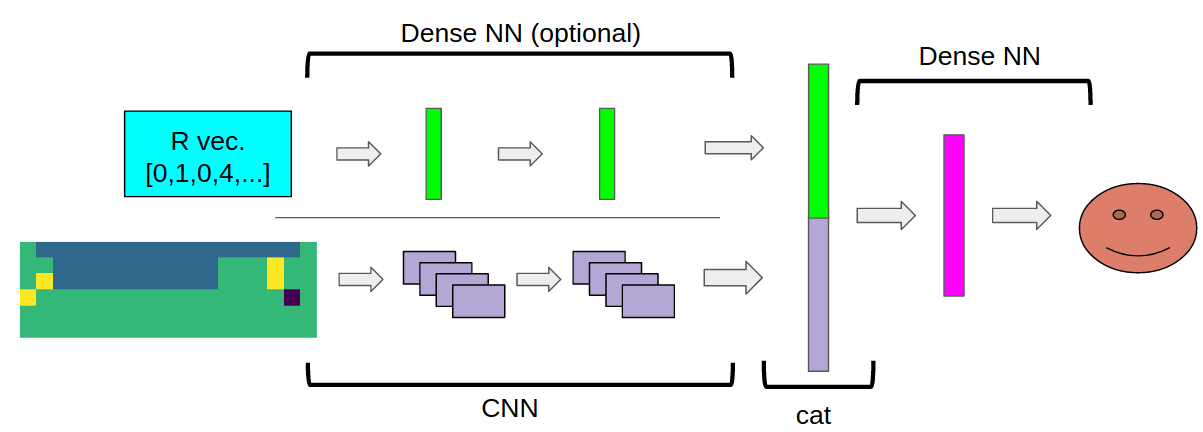
\includegraphics[width=19cm]{CDDNN.png}
\end{figure*}




\renewcommand\refname{Referencias}
\bibliography{bib}
\bibliographystyle{ieeetr}

\end{document}             % End of document.

